\chapter{Binary sequence representation}
\label{kap:kap2}

This chapter is dedicated to outlining the current state of the bit vector
implementations. Bit vector is a data structure storing binary sequence and supporting
methods $\access$, $\rank$ and $\select$. As we have shown in section~\ref{section:WaweletTree},
wavelet tree can be used to build a vector from sequence over the general alphabet
using the bit vector implementation. This is the reason why it is important to dedicate
time to creating fast and efficient bit vector implementation. We start with succinct
representation of bit vector and present ideas to support $\rank$ and $\select$ in sublinear
space. Then we look at the compressed representation of bit vector obtained using the method
introduced by \cite{raman2007succinct}. In the end, we briefly mention the alternative implementations
of compressed bit vector implementation.

\section{Bit vector implementation}

In this section, we introduce practical but also optimal constant time implementations of
$\rank$ and $\select$ methods using the sublinear space overhead.

\subsection{Rank}
\label{section:rank}

Regarding $\rank$ in bit vector, we are concerned with two different methods, namely $\rank_0(i)$
and $\rank_1(i)$. In every binary sequence, it holds that $$\rank_0(i) = i - \rank_1(i).$$
Thus, it is common to only provide the implementation for one of them and answer the other one
using the formula above. Thus, from now on, we consider only $\rank_1(i)$ method and denote
it $\rank$ to simplify notation. There are two straightforward solutions we can begin with to
support $\rank$ on a bit vector~$B$.

The first solution does not use any precomputation at all. Every time we want
to compute $\rank(i)$, we go through all the bits preceding $i$-th and count all
the ones. This solution is not practical for long bit vectors but it does not require
any additional space and precomputation.

The second approach is to precompute $\rank$ of every bit which enables to answer
$\rank$ query in constant time, using a single table lookup. However, the space needed to
support this solution is $\BigO(n\cdot\log n)$ bits, where $n$ is the length of the
bit sequence.

\cite{gonzalez2005practical} combined presented solutions to obtain an idea of a practically
interesting solution where the pre-computed $\rank$ values are stored only for some
bits. At first, we choose a constant $k$ and split bit vector into non-overlapping
subsequences of $k$ bits called \textit{superblocks}. We then precompute $\rank$ only for
the beginning of every superblock. Example of this representation is presented in
Fig.~\ref{obr:practicalRank}. This representation enables answering $\rank$ in time
$\BigO(k)$ as only the precomputed value is accessed and then bits from the start of the
superblock up to the queried position are accessed. This solution uses $\BigO(\ceil{n/k}\log n)$
bits of memory as there are $\ceil{n/k}$ superblocks and every rank stored is at most $n$,
thus taking $\BigO(\log n)$ bits. This version of the implementation allows us to balance between
speed and space usage using the parameter $k$. Increasing parameter $k$ saves space, on the other
hand, smaller $k$ requires less computation to be done inside of the superblock.

In practice, the time of answering the query for smaller $k$ may be dominated by two cache misses
that often occur when answering $\rank$. The first cache miss occurs when accessing precomputed
$\rank$ and the second when accessing the beginning of the superblock. Subsequent linear scan
through superblock is very cache-friendly and thus very fast.

% TODO: moreover, bit operations - popcount
% TODO: in theory, for k ~ log n we already get linear space and \BigO(1) time if we assume a strong-enough model (RAM with log n bit registers with popcount)

\begin{figure}
	\begin{tabular}{c|c|c|c|c|}
	\cline{2-5}
	\textbf{B} & {\tt 0 0 1 0 1 1 0 1} & {\tt 1 1 1 0 1 1 1 1} & {\tt 0 0 0 0 0 1 1 0} & {\tt 1 1 0 0 1} \\ \cline{2-5}
	\end{tabular}

    \bigskip

    \begin{tabular}{c|c|c|c|c|}
        \cline{2-5}
        \textbf{precomputed ranks} & \tt 0 & \tt 4 & \tt 11 & \tt 13 \\ \cline{2-5}
        \end{tabular}

	\caption[TODO]{Example of dividing bit sequence $B$ into superblocks of length 8 and precomputing
    $\rank_1$ for the beginning of every superblock. Note that last superblock may not contain full
    number of 8 bits.}
	\label{obr:practicalRank}
\end{figure}

\paragraph{Constant time rank with sublinear space overhead}

The previous solution works well and is commonly used in practice. However, it is possible to
answer $\rank$ query in constant time with only sublinear space overhead. The constant time
solution is based on partitioning first proposed in this context by \cite{okanohara2007practical}.
As in the previous solution, we start by splitting the bit sequence into superblocks. This time
we set the length of superblock to $\BigO(\log^2 n)$ and again precompute $\rank$s for the beginning of
every superblock. Then, every superblock is further divided into blocks of length $\ceil{(\log n)/2}$.
Similarly to superblocks, for all of these smaller blocks we precompute $\rank$. However, to save space,
we only precompute these $\rank$s from the beginning of the corresponding superblock.

Now, when queried for $\rank$ of some position $i$, we combine:
\begin{enumerate}
    \item $\rank$ precomputed for the beginning of its superblock,
    \item $\rank$ precomputed for the beginning of its block,
    \item $\rank$ inside of its block
\end{enumerate}

The third step can be done also in constant time on unit-cost RAM model with word size $\Theta(\log n)$
that we use in most of our work. We, however, use and analyze here the solution that uses the precomputed table.
This table stores for every possible block and $\rank$ query its result. 

The additional space used by this solution can be broken down into three parts:
\begin{enumerate}
    \item Precomputed $\rank$ for every superblock. Number of superblocks is $\BigO(n/\log^2 n)$
    and we need $\BigO(\log n)$ bits to store every single $\rank$ value so the total amount is
    \begin{equation}
        \BigO\left(\frac{n}{\log^2 n}\cdot \log n\right) = o(n).
        \label{eq:rank_space_1}
    \end{equation}
    \item Precomputed $\rank$ for every block. Number of smaller blocks is $\BigO(n/\log n)$. For every
    block, precomputed $\rank$ from the beginning of a superblock is stored. This value is at most $\log^2 n$,
    thus we need $\BigO(\log\log^2 n)=\BigO(\log\log n)$ bits to store it. The total amount of space is
    \begin{equation}
        \BigO\left(\frac{n}{\log n}\cdot \log\log n\right)=o(n).
        \label{eq:rank_space_2}
    \end{equation}
    \item Precomputed table storing result for every possible $\rank$ query over block. There are only
    $2^{(\log n)/2} = \sqrt{n}$ blocks of length $(\log n)/2$. Number of possible $\rank$ queries over
    block is equal to its length. For every element stored in the table we need at most $\BigO(\log\log n)$
    bits of space so the total amount of space is
    \begin{equation}
        \BigO(\sqrt{n}\cdot \log n\cdot \log\log n)=o(n).
        \label{eq:rank_space_3}
    \end{equation}
\end{enumerate}

The total space used for this solution of $\rank$ is therefore sum of \ref{eq:rank_space_1}, \ref{eq:rank_space_2} and
\ref{eq:rank_space_3}, which is sublinear from $n$.

Even if optimal in theory, this solution is not often used in practice as it produces
3 cache misses and quite complex implementation. One for accessing the precomputed rank up
to the start of the superblock, then another one for the precomputed value of rank to the
beginning of the block and in the end also one for accessing the precomputed $\rank$ value
of the block.

% TODO: ... depends on model... can be \BigO(k/w) if we consider RAM model with w-bit registers
% that supports popcount

\subsection{Select}
\label{section:select}

In case of a $\select$ over bit vector, we are again interested in two methods $\select_0$
and $select_1$. Even if there is not a simple way how to convert the result of one to
another just like with $rank$, we shall be interested mainly in $select_1$ version as the
other one can be implemented using the same ideas. The important property of the $\select$
method is that it works much like an inverse to $\rank$. This is given by the fact that
$$\rank_c(\select_c(i)) = i.$$

Thanks to $\rank$ being a nondecreasing function, it is possible to binary search for the
result of $\select_c(i)$ if we have an efficient implementation of $\rank$. This can be combined
with the solution from the previous section. At first, we binary search for the solution in the
samples of $\rank$ stored in superblocks. After identifying the correct superblock of length $k$
bits, we linearly scan for the result. This solution does not require any additional memory on top
of the space used for $\rank$. The answer is computed in time $\BigO(\log(n/k)+k)$. This solution
even if not optimal works very well in practice as observed by \cite{gonzalez2005practical} on bit
vectors of length up to $2^{20}\approx 10^6$.

\paragraph{Constant time select}

\cite{clark1997compact} proposed solution for $\select$ in a constant time and sublinear space
overhead. The solution is, similarly to the constant time $\rank$ solution, based on a division
to superblocks and blocks.

We begin by precomputing $select(i)$ for every $i$ being multiple of $t_1=\log n\cdot \log\log n$.
These precomputed values take $\BigO(n/\log\log n)$ bits of space. Results of these precomputed
$\select$ queries also split the bit sequence into superblocks of possibly variable length such that
each superblock contains exactly $t_1$ ones (except possibly for the last).

There are now two categories of superblocks. The ones called \textit{long} that are longer
than $t_1^2$. In long superblocks, we can store the positions of all ones as they are sparse
and there is not many of these blocks as they are long. The total space used is $\BigO((n/t_1^2)\cdot t_1\cdot
\log n) = \BigO(n/\log\log n)$.

Dealing with \textit{short} superblocks is harder. On short superblocks, we apply the idea that we
already used for the original bit sequence. Inside of every short superblock, we precompute the
$\select$ from the beginning of the superblock for every multiple of $t_2=(\log\log n)^2$. These
precomputed values are small as they only represent positions from the beginning of a short superblock.
Each of these values takes $\BigO(\log\log n)$ of space so the total amount of space used by these
values is $\BigO(n/t_2\cdot \log\log n) = \BigO(n/\log\log n)$.

This procedure breaks short superblocks into blocks. Again, each of these blocks, possibly except for the
last one contains $t_2$ ones. For blocks longer than $t_2^2$, we store the positions of all
ones as there are not many of these blocks. We may use the same reasoning as in the previous
part to conclude that this takes $\BigO(n/t_2^2\cdot t_2\cdot \log\log n) = \BigO(n/\log\log n)$
of bits.

To deal with the blocks smaller than $t_2^2$ we can again precompute a table of all
the possible ways how the block may look and all the possible $\select$ queries over it with
their result. Number of possible blocks of length $t_2^2$ is equal to $\BigO(2^{t_2^2})$,
number of possible queries over the block is at most its length $t_2^2$ and to store the results
we need roughly $\BigO(\log t_2)$ bits. The table size is thus
$$\BigO(2^{t_2^2}\cdot t_2^2 \cdot \log t_2) = o(n).$$

When answering $select_1(i)$, we can easily find the location of right superblock. If this
is a long superblock, we just look at the precomputed positions of ones in the superblock.
The matter is more complicated if we fall into a short superblock. In this case, we find
the location of the correct block. If this is a long block, we can once again just look
at the position of one we are interested in. If it is a short block, we have the precomputed
table where we index with the block and the position of one in the block, we are interested in.

\section{Compressed representation}
\label{section:compressed_bv}

In the previous section, we showed how $\rank$ and $\select$ queries can be answered in constant
time with just sublinear space overhead. In this section, we show that it is possible to compress
the whole bit vector close to the zeroth order entropy while still keeping the constant time $\rank$
and $\select$.

Up to now, we have been working with straightforward representation of bit vector in which we store
all the bits one after another. This is in general the best thing we can hope for but there are scenarios
where there is a room for improvement. The example is if zeroth order entropy $H_0$ of bit sequence
is small. This occurs in sequences that have very skewed frequency of zeroes or ones. If sequence of
length $n$ has $m$ ones in it, we can store it as before using $n$ bits but there is only ${n \choose m}$
such sequences and it may be more beneficial for big $m$ to store the sequence number which one of these
we are working with. It is possible to prove for sequence $S$ of length $n$ with $m$ ones that
$$\lg {n \choose m} = nH_0(S)+\BigO(\log n).$$ This means that using this representation may be
beneficial in scenarios when $nH_0(S)\ll n$.

This is an idea that RRR is based on. RRR is a data structure based partly on the work of \cite{pagh2001low}
and proposed by \cite{raman2007succinct}. The main idea of RRR is to split the bit sequence into blocks of size
$b$ and then represent a block with $c$ ones using only $\ceil{\log {b \choose c}}$ bits as
there are ${b \choose c}$ combinations for positions of ones. The whole block can be then uniquely
represented as a pair $(c, o)$ where $c$ is the number of ones in the block, called \emph{class} and
$o$ is an \emph{offset} of this block in a sequence of all the ${b \choose c}$ blocks in this particular class.
Even if the ordering of the blocks with the same class can be arbitrary, only lexicographical ordering
is heavily used in practice.

Now, for this structure to work, we need to find a way how to convert between the bit representation of
a block and its compressed form $(c, o)$. The process of obtaining $c$ and $o$ from the raw representation
of block is called \textit{encoding}. The opposite process is called \textit{decoding}. We would like both
processes to be fast, however, in most of the applications where bit vector is used, we do the encoding only
once at the initial construction of the bit vector. Decoding, on the other hand, is done every time we are
accessing a particular bit in $B$. Thus, in practice, it is more important to optimise the speed of decoding.

\paragraph{Block encoding/decoding}

For shorter block lengths, such as $b\leq 15$, it is reasonable to generate two helper tables $E$ and $D$.
Table $E$ used for the encoding, maps the block to its offset. The other table $D$ is two dimensional and
stores the bit representation of the block that is associated with pair $(c, o)$ on position $D[c][o]$.
Both these tables $E$ and $D$ can be precomputed by generating all the possible blocks in lexicographical
order. After this precomputation, the encoding and decoding of a block takes constant time.

For longer blocks, it is impractical or even impossible to store huge helper tables. On the other
hand, bigger block sizes yield better compression rates because of smaller per block overhead. \cite{navarro2012fast}
developed method we shall call \textit{on the fly-decoding}, that does not require these big helper tables. 
This method relies on a bit by bit encoding and decoding of the block, taking $\BigO(b)$ time. While decoding,
we can compute on every position using simple combinatorics, how many blocks precede a given prefix and decide,
whether next bit should be 0 or 1. Pseudocode of this idea computing binary representation of block is in
listing~\ref{alg:on_the_fly}.

\begin{algorithm}
\caption{Pseudocode for on-the-fly decoding}\label{alg:on_the_fly}
    \KwData{$c, o$}
    $block \gets 0$\;
    \For{$i=0$ \KwTo $b-1$} {
        \tcp{$p$ is number of blocks with same prefix and zero on $i$-th position}
        $p \gets {b-i-1\choose c}$\;
        \If{$o<p$} {
            \tcp{add zero at the end of the block}
            $block \gets 2\cdot block$\;
        } \Else {
            \tcp{add one at the end of the block}
            $block \gets 2\cdot block+1$\;
            $c \gets c-1$\;
            $o \gets o-p$\;
        }
    }
    \KwRet{$block$}
\end{algorithm}

On the fly decoding does not use helper tables $E$ and $D$ but to achieve the best possible time complexity
it requires the precomputation of combination numbers it uses. These, however, use together less than $\BigO(b^3)$
of bits

\paragraph{Arrangement of encoded blocks}

In the previous paragraph, we showed how single block can be encoded and decoded. The next question is how the
encoded pairs representing blocks are arranged in memory. This arrangement should consider space efficiency
but also allow easy access to individual blocks of $B$. 

The main part of this representation comprises of two arrays $C$ and $O$ storing the classes and offsets of
the blocks, respectively. The array $C$ is an array of elements that are of fixed length. Every element takes
$\lg (b+1)$ bits of space. The array $O$, on the other hand, is an array of elements of variable
size where the $i$-th element is $\lg {b\choose C[i]}$ bits long. Note that accessing $i$-th element
in array $C$ is easier than doing the same in array $O$.

\paragraph{Accessing bits in RRR}

Accessing $x$-th bit of original sequence $B$ consists of three steps. The first is to obtain the
compressed representation of a block where $x$-th bit is located. The second step is to decode this block and
the third is to access the particular bit of interest in the decoded block. The $x$-th bit is contained in the
$i$-th block where $i=\floor{x/b}$. Its compressed representation is $(C[i], O[i])$.

Obtaining $C[i]$ is trivial as it is at the fixed memory offset from the beginning of array $C$. Getting the
value of $O[i]$ is harder as it is not at a known memory offset but it can be still expressed as
$$\sum_{j=1}^{i-1} \lg {b\choose C[j]}.$$ This can not be, however, computed in constant time without
any precomputed information and we need to basically one by one skip over elements that come before $O[i]$.
To access the $i$-th block, we need in the worst case to look at all the elements of $C$ and this
takes $\BigO(n/b)$ time. For now, we stay with this solution and analyze its space usage.

\paragraph{Space usage of RRR}

Our current representation needs to store the arrays $C, O$ and helper table $D$. Let us now
analyze the space used by these structures. $C$ is an array of $\ceil{n/b}$ elements of fixed size
$\lg (b+1)$. For array $O$ we argue that its size is bounded by

\begin{align*}
    \sum_{i=1}^{n/b} \lg {b\choose c_i}
    &\leq \sum_{i=1}^{\ceil{n/b}} \log_2 {b\choose c_i} + \ceil{n/b} \\
    &= \log_2\prod_{i=1}^{\ceil{n/b}} {b\choose c_i} + \ceil{n/b} \\
    &\leq \log_2{n\choose \#_1(B)} + \ceil{n/b} &\leq nH_0(B) + \ceil{n/b}
\end{align*}

where $\#_1(B)$ denotes the total number of ones in $B$. The second inequality was obtained using
the observation that ${n\choose k} {m\choose \ell} \leq {n+m\choose k+\ell}$. This can be seen
when we interpret the left side of the equation as a number of ways we can choose $k$ elements
from $n$ elements and $\ell$ elements from another $m$ elements. This is all contained on the
right side of the equation that includes all these combinations. $D$ is storing $2^b$ entries
and each entry is using $b$ bits of storage. The total space used is then
$$nH_0(B) + \ceil{n/b} + \ceil{n/b} \cdot \lg(b+1) + b2^b.$$

\paragraph{Block access speed up}

To speed up the process of accessing block, we can store the pointers into every $k$-th element
of $O$. This again creates some bigger superblocks as can be observed in Fig.~\ref{obr:RRRFinal}.
This representation speeds up the process of locating offset $O[i]$. Now, we at first find the
nearest pointer leading to superblock where $i$ is located and then we just skip through superblock
at most $k$ times to locate $O[i]$. This additional structure of $\floor{n/(bk)}$ integers uses
$\BigO(\log(n)\cdot \frac{n}{bk})$ bits of space.

\begin{figure}
	\centerline{
		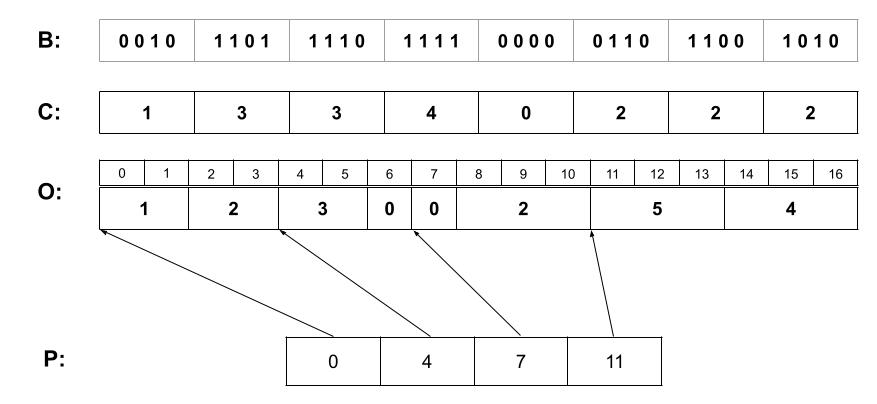
\includegraphics[width=0.9\textwidth, height=0.3\textheight]{images/rrr}
	}
	\caption[TODO]{RRR implementation. $B$ shows the original bit sequence cut to
    blocks. $C$ stores the class which is in this case number of ones in the block.
    $O$ uses variable number of bits per entry, in general, $i$-th entry uses
    $\lg {b\choose C[i]}$ bits and stores the lexicographical order
    of this block in the class $C[i]$. For $k=2$ we can see a helper array $P$
    storing bit offsets into every $k$-th element namely $0, 2, 4\ldots$
	}
	\label{obr:RRRFinal}
	% source at https://docs.google.com/drawings/d/1f1M7e-dZIiIZh1RdgqnmptF3xWZBKqjms3f_aQwVMhg/edit
\end{figure}

When setting the block size to $\log(n)/2$ we obtain interesting practical results as
the total space used by our representation is equal to $nH_0(B) + o(n)$ bits. This means
that we are storing only a sublinear amount of data on top of the zeroth order empirical entropy.

When we are interested in obtaining the best practical results, block size becomes
one of the most important parameters of RRR implementation. As we shall show in the next
chapter, bigger block size is better because of lower per bit overhead. Also, not all block
sizes are used in practice. Very often, we are interested in block sizes of the form $2^k-1$.
This is because the number of ones in block of size $2^k-1$ can be number between 0 and $2^k-1$
making this in total $2^k$ possibilities. Storing this number in the fixed bucket of size
$k$ bits makes use of all the available space. This is why most commonly used bucket sizes in
practice are 15, 31, 63 and 127. For block size of 15 the encoding and decoding table
each occupies roughly 64kB of space. This is because every table consists of $2^{15}$ of entries
each taking 2 bytes of storage. Unfortunately, for block size of 31 these two tables would consume
roughly $2^{31}\cdot 4$ bytes of storage. That amounts to roughly 8.5GB of space and makes this approach
unusable in practice. This problem force us to use the on the fly decoding for block sizes
bigger than 15. The disadvantage of this approach is that it takes $\BigO(b)$ steps to decode the block.
Furthermore, on the fly decoding contains branches and it is hard to parallelize its steps in some meaningful
way. Overall, this makes the block size a parameter that we can adjust to balance between better space
efficiency and faster runtime performance.

\paragraph{Alternatives}
% https://github.com/simongog/sdsl-lite/blob/master/include/sdsl/sd_vector.hpp

So far we have provided just one example of the bit vector implementation.
RRR is used on sequences with low entropy, where the frequency of zeroes/ones
is shifted to one or the other side such as 20-40\% of all bits are the same.
There is also a second class of the bit vector implementations, heavily
used when the frequency of zeroes or ones is more significantly shifted.
We stated that RRR is used in case of shifted frequencies, but when the number
of ones is very small, e.g. less than 5\% of the sequence, sparse bit vector
implementations may outperform solutions based on RRR as was observed by \cite{navarro2012fast}.
Where RRR stands out from some of its alternatives is that it is also very competitive
in cases where frequencies of zeroes and ones are similar globally, but the bit
sequence has a lot of places where locally zeroes or ones are over-represented.
Numerous sparse bit vector solutions are based on the work of \cite{okanohara2007practical}.